\documentclass[conference]{IEEEtran}
\IEEEoverridecommandlockouts
\usepackage{cite}
\usepackage{amsmath,amssymb,amsfonts}
\usepackage{graphicx}
\graphicspath{{../figs/}}
\usepackage{textcomp}
\usepackage{xcolor}
\usepackage{booktabs}
\usepackage{url}
\usepackage{amsthm}
\newtheorem{proposition}{Proposition}
\renewcommand{\topfraction}{0.95}
\renewcommand{\bottomfraction}{0.95}
\renewcommand{\textfraction}{0.05}
\renewcommand{\floatpagefraction}{0.9}
\renewcommand{\dbltopfraction}{0.95}
\renewcommand{\dblfloatpagefraction}{0.9}
\def\BibTeX{{\rm B\kern-.05em{\sc i\kern-.025em b}\kern-.08em
    T\kern-.166em\lower.7ex\hbox{E}\kern-.125emX}}

\begin{document}

\title{Clause-Activation Signatures (CAS) for Attack-Family Attribution in IoMT}

\author{Rakesh Reddy Yakkati, Per-Arne Andersen, Lei Jiao, Ole-Christoffer Granmo, and Rishad Shafik
\thanks{This work was supported by the \textit{SecureIoTM---Ultra-low-energy IoT Intrusion Detection Systems using Logic-based Tsetlin Machines} project (Grant Number 342167), funded by the Research Council of Norway under the TEKNOLOGIKONVER programme. The authors acknowledge the support from the Centre of Artificial Intelligence Research at the University of Agder, Sørlandet Hospital Trust, and Newcastle University for their collaboration in this interdisciplinary research initiative.}% <-this % stops a space
\thanks{Rakesh Reddy Yakkati, Lei Jiao, and Ole-Christoffer Granmo are with the Department of ICT, University of Agder, Grimstad 4879, Norway (emails rakeshry@uia.no, lei.jiao@uia.no, and ole.granmo@uia.no).}
\thanks{Per-Arne Andersen is with the Department of Information Systems, University of Agder, Kristiansand 4630 (email per.andersen@uia.no).}
\thanks{Rishad Shafik is with the Department of Microelectronic Systems, Newcastle University, Newcastle upon Tyne, UK (email rishad.shafik@newcastle.ac.uk).}}

\maketitle

\begin{abstract}
When an intrusion detector flags traffic in the Internet of Medical Things
(IoMT), a label alone is not enough --- the analyst must also know
\emph{which} attack family is at play and \emph{why}. This paper introduces
Clause-Activation Signatures (CAS), a method that turns the clauses of a
trained weighted Tsetlin Machine (TM) into a compact, auditable signature
for each attack family, so that attribution becomes signature matching
rather than an opaque vote. Each signature is extracted with
complementary-pairs stability selection (CPSS) over clause activations,
split by coefficient sign into inculpatory and exculpatory evidence, and
certified by a Shah--Samworth bound on spurious inclusions. Evaluated on
CICIoMT2024 (WiFi/MQTT, family level) across three independently seeded
TMs, CAS attribution improves over the raw weighted-vote TM it is extracted
from: macro-F1 rises from $0.692 \pm 0.004$ to $0.765 \pm 0.029$ at the
verified operating point, using only 28--53 sign-positive clauses per
family out of a 2{,}400-clause pool. Sorting each class's clauses by
weight and discarding the weakest $84\%$ before extraction costs the base
detector nothing, lifts CAS to $0.779 \pm 0.025$, and removes its
sensitivity to the stability threshold entirely. The six signatures
provably form a
maximally 5-disjunct code on every seed, so any mixture of up to five
families decodes exactly; under 5\% bit-flip noise a thresholded decoder
still recovers 99.8\%--100\% of mixtures. A binary normal-versus-attack
reduction lifts AUROC from 0.819 to 0.940. Two honest negative results are
reported: open-set novelty detection is weak under correct
conformal false-flag control, and signature identity does not survive
retraining under a different seed. CAS is thus a
certified attribution and interpretability layer that denoises a mediocre
base detector, not as a replacement for one.
\end{abstract}

\begin{IEEEkeywords}
Tsetlin Machine, interpretable machine learning, intrusion detection, IoMT,
stability selection, disjunct codes, attack attribution, open-set
recognition
\end{IEEEkeywords}

\section{Introduction and Related Work}
Intrusion detection for the Internet of Medical Things (IoMT) must satisfy
two requirements simultaneously: the alarm must be correct, and it must
identify the responsible attack family in a form a forensic analyst can
audit, since the appropriate response differs fundamentally across families
and patient safety can depend on the distinction. Existing IDS
explainability does not meet the second requirement. Post-hoc explainers
such as SHAP, LIME, and Anchors~\cite{xaiids2025} account for one
prediction at a time and provide no stability guarantee: retraining the
model or perturbing the explainer changes the explanation. A per-family
\emph{signature} --- a small rule set that is interpretable by design,
vetted for stability, and attached to a family rather than to a single
flow --- remains absent from the literature.

A candidate substrate for such signatures is the Tsetlin Machine
(TM)~\cite{granmo2018}, whose unit of computation is a conjunctive clause
over Boolean literals learned through bandit-driven Type~I/II feedback;
clauses remain human-readable after training, and the weighted
TM~\cite{phoulady2020} preserves this property while learning an integer
vote weight per clause. TM-based intrusion detection is established:
Abeyrathna et al.\ extracted interpretable TM rules on
KDD'99/NSL-KDD~\cite{abeyrathna2020}, and Jaiswal et al.\ trained TMs on
CICIoMT2024, reporting 90.7\% six-class accuracy~\cite{jaiswal2026iomt}
and 97.8\% macro-F1 on MedSec-25~\cite{jaiswal2026medsec}. These works,
however, explain individual predictions through whichever clauses happened
to fire; they do not aggregate activations into stable per-family
signatures, and they provide no error control on the explanation.

This paper closes that gap with Clause-Activation Signatures (CAS) for
attack-family attribution. A trained weighted TM maps every flow to a
vector of clause activations. For each family $\ell$, CAS selects the
clauses whose activations are stably predictive of $\ell$ using
complementary-pairs stability selection (CPSS)~\cite{shah2013} over the
clause-activation space, and splits the selection by coefficient sign into
inculpatory and exculpatory evidence. Because CPSS is governed by the
Shah--Samworth bound, each signature carries a certificate on the expected
number of spurious inclusions. Attribution then reduces to signature
matching: a flow is attributed to the family whose signature it matches
best, and the matched clauses are the explanation returned to the
analyst.

The construction rests on two bodies of theory. The first is stability
selection~\cite{meinshausen2010,shah2013}, applied here to clause
activations rather than raw features; to our knowledge this usage, and
clause-level forensic security signatures generally, are new. The second
is $t$-disjunct matrices from combinatorial group testing~\cite{du1993}:
if no column of a binary incidence matrix is covered by the union of any
$t$ other columns, any mixture of at most $t$ columns decodes exactly.

The evaluation requires a dataset that survives standard IDS validity
criteria~\cite{sommer2010,engelen2021,arp2022}. CICIoMT2024~\cite{dadkhah2024}
is the only peer-reviewed, widely adopted IoMT-specific benchmark spanning
multiple protocols, and its schema contains no IP or port fields, removing
the most common leakage channel by design.

The contributions are: (1) a correctness-audited, seed-reproducible CAS
implementation on TMU~\cite{tmu} clause activations, including a
sign-filtering fix without which attribution falls below the base detector
(\S\ref{sec:cpss}, \S\ref{sec:validation}); (2) a three-seed verified
evaluation showing CAS outperforms its base TM above a stability threshold
we identify (\S\ref{sec:taska}); (3) signed, human-readable evidence lists
per family with an explicit error-control certificate
(\S\ref{sec:signatures}); (4) an exact disjunct-code certificate, maximal
on all seeds, where the decoder rather than the code is the noise
bottleneck (\S\ref{sec:disjunct}); (5) a binary normal-versus-attack
reduction where the attack signature markedly improves detection ranking
(\S\ref{sec:binary}); and (6) two negative results: weak open-set novelty
power under correct conformal false-flag control (\S\ref{sec:taskb}), and
near-chance cross-seed signature identity (\S\ref{sec:stability}).

\section{Method: Clause-Activation Signatures}
\subsection{Overview}
Fig.~\ref{fig:cpss} shows the core stages involved in
detail for the proposed method.Initially, the raw flows are binarized using exisiting standard binarizer in TMU library. Then, a weighted TM is trained on them. Then the final output of the TM is its learned rules (clauses that fire on it). The purpose of CPSS is to extracts a stable
clauses per class. In this process, two stages accompany
the clasuses: a statistical error-control bound and a combinatorial
identifiability guarantee.

\begin{figure*}[t]
\centering
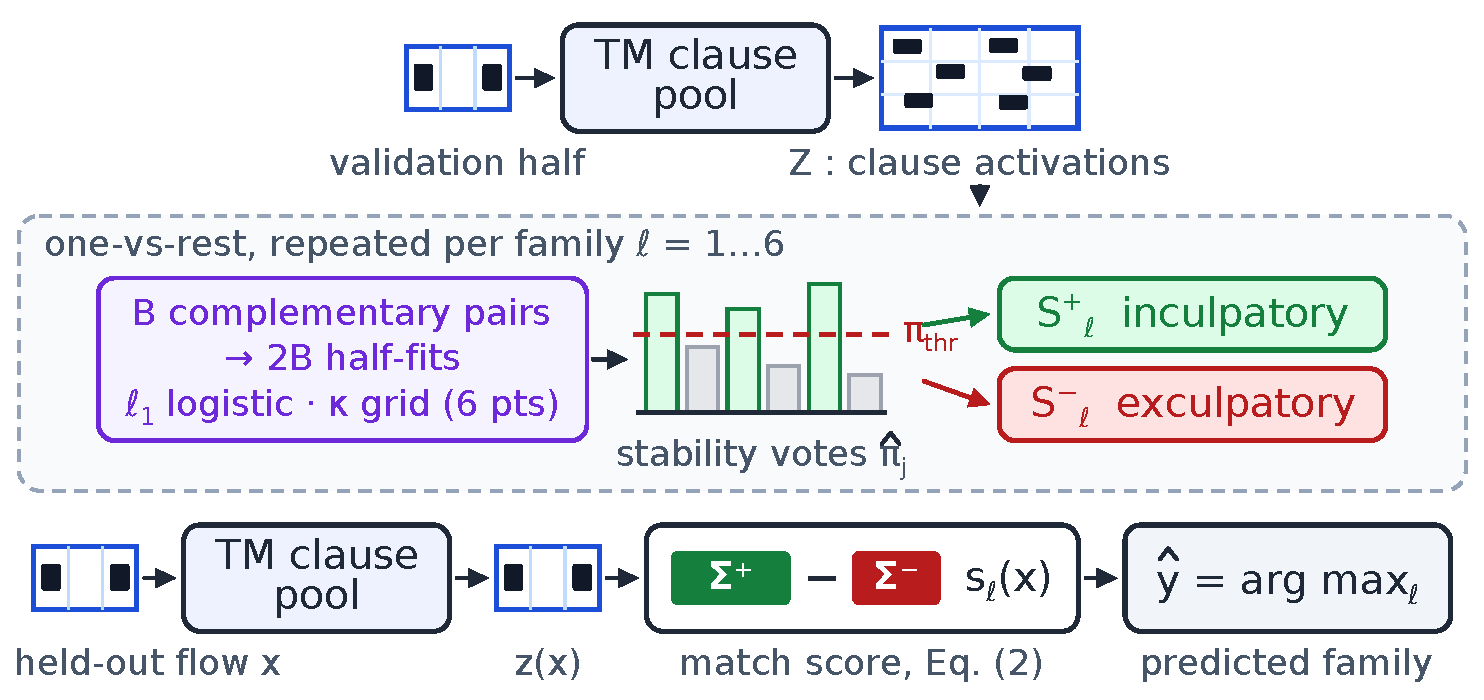
\includegraphics[width=0.32\textwidth]{fig_cpss.pdf}
\caption{CPSS signature extraction and sign filtering. CPSS votes on
clauses across $2B$ complementary half-fits (a $\kappa$ grid per fit),
thresholds the votes at $\pi_{\mathrm{thr}}$, and splits each signature by
coefficient sign into inculpatory $S_\ell^{+}$ and exculpatory $S_\ell^{-}$
evidence for scoring.}
\label{fig:cpss}
\end{figure*}

\subsection{Dataset Description}
We use CICIoMT2024~\cite{dadkhah2024}, WiFi/MQTT branch, with family-level
labels. The dataset was collected on a testbed of 40 healthcare devices
(25 real, 15 simulated) communicating over Wi-Fi, MQTT, and BLE. It
contains 18 attack types grouped into five families, and each flow is
described by 22 numeric CIC-extracted flow features. The six families are
Benign, distributed denial-of-service (DDoS),
denial-of-service (DoS), attacks on the Message Queuing Telemetry Transport
protocol (MQTT), reconnaissance (Recon), and Spoofing.
\subsection{Booleanization and Base Detector}
\label{sec:bool}
Each numeric flow feature is discretized into 10 quantile bins. We use
scikit-learn's KBinsDiscretizer with bin edges fit on the training
partition only. The bins are encoded as cumulative thermometer bits of the
form ``feature $\ge$ bin $k$''. TMU handles literal negation internally.
\subsection{WTM}
We train a weighted multiclass TM on the six
classes with 400 clauses per class, $T=320$, $s=8.0$, and 25 epochs.
Since, the dataset has six attack-family classes. Passing
flows through the trained TM, with 400 clauses learned per class, yields
the clause-activation matrix $Z \in \{0,1\}^{n \times 2400}$. Here
$Z[x,j]=1$ if and only if clause $j$ fires on input $x$.

\subsection{Clause-Pool Pruning}
\label{sec:prune}
Not every clause in the pool is worth carrying into signature extraction,
and which ones to drop can be posed exactly. Write $w_{c,j}$ for the
learned weight of clause $j$ of class $c$ and $z_{c,j}(x) \in \{0,1\}$ for
its activation, so the class sum is $f_c(x)=\sum_j w_{c,j} z_{c,j}(x)$ and
$\hat{y}(x)=\arg\max_c f_c(x)$. A keep-mask
$m \in \{0,1\}^{C \times n}$ with deletion sets $D_c=\{j: m_{c,j}=0\}$
gives $f_c(x;m)=\sum_j m_{c,j} w_{c,j} z_{c,j}(x)$, and we seek the
smallest pool that preserves accuracy:
\begin{equation}
\min_{m \in \{0,1\}^{C \times n}} \lVert m \rVert_0
\quad\text{s.t.}\quad
\mathrm{F_1}\!\left(\hat{y}(\cdot\,;m)\right) \ \ge\
\mathrm{F_1}\!\left(\hat{y}(\cdot\,;\mathbf{1})\right) - \varepsilon .
\label{eq:prune}
\end{equation}
This is a search over $2^{Cn}$ masks ($2^{2400}$ here) whose constraint is
non-decomposable, macro-F1 sitting behind an $\arg\max$. We therefore
optimise the perturbation it induces,
$R(D_c) := \sum_{j \in D_c} |w_{c,j}|$, which controls~\eqref{eq:prune} through the
decision margin.

\begin{proposition}[Certificate]
\label{prop:cert}
Let $R = \max_c R(D_c)$ and let
$\gamma(x)=f_{\hat{y}(x)}(x)-\max_{c \neq \hat{y}(x)} f_c(x)$ be the
full-pool margin. If $\gamma(x) > 2R$ then $\hat{y}(x;m)=\hat{y}(x)$.
\end{proposition}
\begin{proof}
Since $z_{c,j}(x) \in \{0,1\}$,
$|f_c(x)-f_c(x;m)| = |\sum_{j \in D_c} w_{c,j} z_{c,j}(x)| \le R(D_c) \le R$
for every $c$. Writing $a=\hat{y}(x)$, for any $c \neq a$,
$f_a(x;m)-f_c(x;m) \ge \bigl(f_a(x)-R\bigr)-\bigl(f_c(x)+R\bigr)
\ge \gamma(x)-2R > 0$, so $a$ remains the maximiser.
\end{proof}

\begin{proposition}[Exact greedy]
\label{prop:greedy}
For a budget $|D_c| = k$, $\min_{D_c} R(D_c)$ is attained by the $k$
clauses of smallest $|w_{c,j}|$.
\end{proposition}
\begin{proof}
$R(D_c)$ is a sum of $k$ non-negative terms selected without replacement.
If $D_c$ contains $j$ while excluding $j'$ with $|w_{c,j'}| < |w_{c,j}|$,
swapping them strictly decreases $R$; no such swap exists precisely when
$D_c$ holds the $k$ smallest magnitudes.
\end{proof}

Magnitude ranking is therefore optimal for the surrogate rather than a
heuristic, and by Proposition~\ref{prop:cert} it carries a per-input
guarantee, at cost $O(Cn\log n)$ against the $2^{Cn}$ of~\eqref{eq:prune}. Sweeping
$k$ in steps of five and taking the largest $k$ that meets the constraint
gives the operating budget used in \S\ref{sec:pruned}; CAS is then
extracted from the surviving pool exactly as below, with nothing else
changed.

\subsection{CPSS Signature Extraction and Sign Filtering}
\label{sec:cpss}
CAS works entirely
in clause activation space, where a flow is represented by the rules that match it. We build one one-versus-rest problem
per family $\ell$. CPSS then repeats the following procedure $B$ times. It
splits a validation half of the test set into two complementary halves. On
each half it fits an $\ell_1$-regularized logistic model. The features of
this model are the clause activations, i.e., the columns of $Z$. The target
is the one-versus-rest label of family $\ell$. This yields $2B$ half-fits
per family.

Two knobs control this stage. The first is $\kappa$. It is the
inverse-regularization strength of the logistic model inside each half-fit.
The second is $\pi_{\mathrm{thr}}$. It is the stability threshold applied
after all fits are done. The knob $\kappa$ sets how sparse one single fit is. A small $\kappa$
forces most coefficients to exactly zero. Each coefficient belongs to one
clause. Only a few clauses then survive a single half-fit. We do not fix one $\kappa$. We sweep it over a geometric
grid of 6 points from 0.001 to 0.1. A clause counts as selected by a
half-fit if any grid point selects it. This union-over-grid rule
follows~\cite{shah2013}.

Each half-fit casts one vote per clause. The stability score
$\hat{\pi}_j$ is the fraction of the $2B$ half-fits that select clause $j$.
The signature keeps the clauses that win enough votes:
$S_\ell = \{j : \hat{\pi}_j \ge \pi_{\mathrm{thr}}\}$. So
$\pi_{\mathrm{thr}}$ sets how consistent a clause must be across votes. The two knobs are not independent. $\kappa$ sets which clauses can collect
votes at all. $\pi_{\mathrm{thr}}$ then cuts the resulting vote
distribution. A denser $\kappa$ grid lets more clauses survive each fit.
More clauses then pass any fixed $\pi_{\mathrm{thr}}$. So the signature
size at a given threshold depends on the grid. A low $\pi_{\mathrm{thr}}$ threshold admits clauses that barely pass
half of the fits. A higher threshold
keeps only clauses that nearly every fit selects. We restrict $\kappa$ to the range that keeps each half-fit sparse on this
2{,}400-clause pool. A wider grid would inflate $q_\Lambda$ and make the
certificate vacuous.

One further step is needed. CPSS selects on $|$coefficient$|>0$. This is
correct for the error-control bound. It is wrong for attribution. A stably
negative coefficient is evidence \emph{against} $\ell$ and not for it. We
therefore track the mean signed coefficient
$\overline{\mathrm{coef}}_j$ of each clause across fits. We split the
signature into
$S_\ell^{+} = \{j \in S_\ell : \overline{\mathrm{coef}}_j > 0\}$
and $S_\ell^{-}$. The positive part is inculpatory evidence. The negative
part is exculpatory evidence. The certificate still applies to the full
sign-agnostic $S_\ell$. We state this scoping gap openly.
\S\ref{sec:validation} shows that this split is not cosmetic.

The attribution score is
\begin{equation}
s_\ell(x) = \frac{\sum_{j \in S_\ell^{+}} \hat{\pi}_j z_j(x) - \sum_{j \in S_\ell^{-}} \hat{\pi}_j z_j(x)}{\sum_{j \in S_\ell^{+}} \hat{\pi}_j},
\label{eq:score}
\end{equation}
and the prediction is $\hat{y} = \arg\max_\ell s_\ell(x)$. Matches to
inculpatory clauses add weight. Matches to exculpatory clauses subtract
weight. Normalization by the inculpatory weight is required. Without it
scores scale with signature size instead of match quality.

\subsection{Error-Control Certificate}
\label{sec:cert}
With $q_\Lambda$ estimated as $\mathrm{mean}(\hat{\pi}) \cdot p$, the
Shah--Samworth bound gives
$E[V] \le q_\Lambda^2 / ((2\pi_{\mathrm{thr}} - 1) p)$ with $p = 2400$. We
report these bounds as loose wherever they are loose
(\S\ref{sec:signatures}). They certify that most of each signature is
likely genuine. They do not certify that it is near-noise-free.

\section{Experimental Setup}
\label{sec:setup}
 We apply stratified caps for tractability. Each family
contributes at most 40{,}000 training and 15{,}000 test rows. Benign
(19{,}291 rows) and Spoofing (16{,}047 rows) are used in full. This yields
195{,}338 training and 80{,}868 test rows. The raw distribution is heavily
imbalanced, with DDoS and DoS together accounting for about 95.7\% of
flows~\cite{dadkhah2024}. We therefore report macro-F1 and per-class
metrics throughout.

Signatures are constructed with CPSS on a random half of the test set and
evaluated on the disjoint remaining half, so no leakage occurs between
signature fitting and evaluation. Multi-seed results use three
independently trained TMs with seeds 42, 7, and 123 and fully seeded CPSS.

\section{Results}
We proceed from construction checks
(\S\ref{sec:validation}) to closed-set family attribution
(\S\ref{sec:taska}), its sensitivity to the CPSS knobs
(\S\ref{sec:sweep}) and its binary reduction (\S\ref{sec:binary}), the
signatures themselves (\S\ref{sec:signatures}) and what happens when the
clause pool is pruned first (\S\ref{sec:pruned}), open-set behavior
(\S\ref{sec:taskb}), mixture identifiability
(\S\ref{sec:disjunct}), and cross-seed stability (\S\ref{sec:stability}).

\subsection{Validation of the Construction}
\label{sec:validation}
Three checks validate the construction.
First, the \texttt{Rate}-clipping fix
(\S\ref{sec:bool}) is essential: without it, macro-F1 collapses from 0.72 to
0.54. Second, the sign split
(\S\ref{sec:cpss}) is not cosmetic: a naive sign-agnostic scorer reaches
only 0.642--0.666 macro-F1 --- \emph{below} the 0.686 TM-argmax baseline
--- while the signed scorer reaches 0.719--0.776, comfortably above it. Third, $\pi_{\mathrm{thr}}=0.6$ is unstable: reruns score as low as
0.638--0.643 with cross-seed standard deviation 0.028--0.032, roughly
twice the 0.015--0.022 at $\pi_{\mathrm{thr}} \ge 0.7$; at 0.8
the selected set is stably separated. We therefore report
$\pi_{\mathrm{thr}}=0.8$ as the verified operating point throughout.
\subsection{Task A: Closed-Set Family Attribution}
\label{sec:taska}
Table~\ref{tab:headline} gives the verified three-seed headline results:
at the verified threshold CAS beats its base detector on every seed, with
smaller signatures than at lower thresholds; raising $B{=}15$ to
$B{=}25$ and fusing with the raw TM vote add nothing further.

\begin{table}[t]
\centering
\caption{Task A: verified three-seed macro-F1 on CICIoMT2024.}
\label{tab:headline}
\small
\begin{tabular}{@{}lcc@{}}
\toprule
Method & $B{=}15$ & $B{=}25$ \\
\midrule
Weighted-TM argmax (base) & $0.692 \pm 0.004$ & (same models) \\
CAS $\pi_{\mathrm{thr}}{=}0.6$ & $0.688 \pm 0.032$ & $0.678 \pm 0.028$ \\
CAS $\pi_{\mathrm{thr}}{=}0.7$ & $0.743 \pm 0.015$ & $0.737 \pm 0.022$ \\
\textbf{CAS $\pi_{\mathrm{thr}}{=}0.8$} & $\mathbf{0.765 \pm 0.029}$ & $0.750 \pm 0.034$ \\
CAS $\pi_{\mathrm{thr}}{=}0.9$ & $0.762 \pm 0.038$ & $0.761 \pm 0.038$ \\
Fusion (TM + CAS, $\lambda$ on val) & $0.764 \pm 0.010$ & $0.768 \pm 0.013$ \\
\bottomrule
\end{tabular}
\end{table}

The gains come from where the base detector is weakest: in the recorded
primary run (seed 42, $\pi_{\mathrm{thr}}{=}0.6$,
$B{=}15$), Benign recall rises from 0.30 to 0.64 and Spoofing precision
from 0.41 to 0.55 (Fig.~\ref{fig:taska_recall}). DDoS and
DoS, by contrast, stay mutually confused under both methods, with
near-identical F1 --- a documented dataset
property~\cite{domenech2025}, not a signature-quality artifact.

\begin{figure}[!t]
\centering
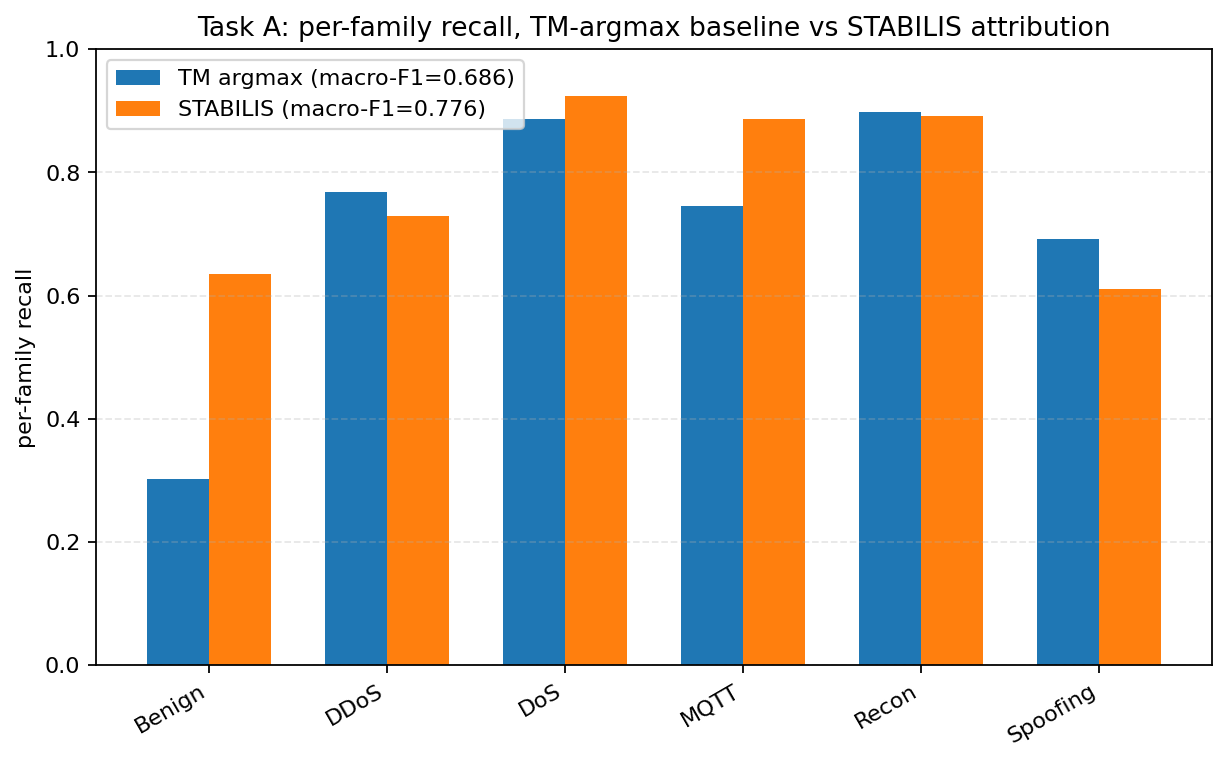
\includegraphics[width=0.40\columnwidth]{task_a_per_family_recall.png}
\caption{Per-family recall, base weighted-TM argmax versus CAS
attribution; the gains concentrate on Benign and Spoofing.}
\label{fig:taska_recall}
\end{figure}

\subsection{Sensitivity to $\pi_{\mathrm{thr}}$, $B$, and $\kappa$}
\label{sec:sweep}
Fig.~\ref{fig:sweep} sweeps the two CPSS knobs and the number of
complementary pairs, on the same three seeds and the same evaluation half
as Table~\ref{tab:headline}. Both metrics tell the same story about
$\pi_{\mathrm{thr}}$: at $0.5$--$0.6$ CAS sits at or below the base
detector (macro-F1 $0.708$/$0.688$ vs.\ $0.692$; accuracy $0.731$/$0.712$
vs.\ $0.726$), from $0.7$ it clears the base on both, and it peaks at
$\pi_{\mathrm{thr}}{=}0.8$ ($0.765$ macro-F1, $0.783$ accuracy) --- the
operating point adopted throughout. The number of complementary pairs
matters much less: macro-F1 rises from $0.738$ at $B{=}5$ to $0.765$ at
$B{=}15$ and is flat thereafter ($0.750$ at $B{=}20$ and $B{=}25$), so
$B{=}15$ already saturates the stability estimate and every setting stays
above the base detector.

The regularization strength is the least sensitive knob
(Table~\ref{tab:grid}): across two orders of magnitude,
$\kappa \in [10^{-3}, 4\times10^{-2}]$, the three-seed mean varies only
between $0.725$ and $0.764$, and it is only at $\kappa{=}0.1$ --- where
single half-fits stop being sparse --- that CAS degrades toward the base
detector ($0.674$--$0.722$). This is what justifies the union-over-grid
rule of \S\ref{sec:cpss}: at the verified threshold the union
($0.765$) beats every individual grid point (best single $\kappa$:
$0.752$), so pooling the grid recovers clauses no single sparsity level
selects on its own.

\begin{figure}[!t]
\centering
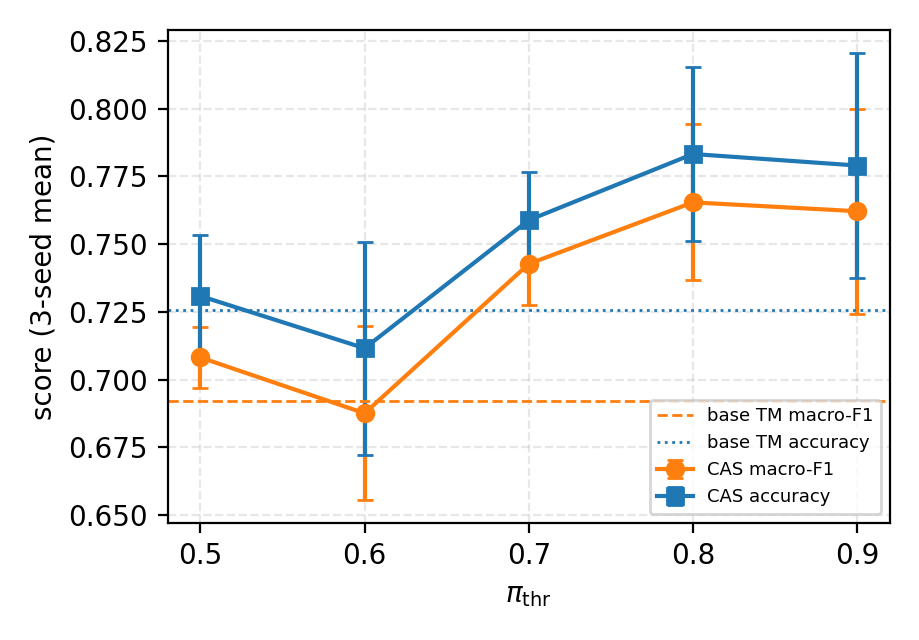
\includegraphics[width=0.49\columnwidth]{old_pithr.png}\hfill
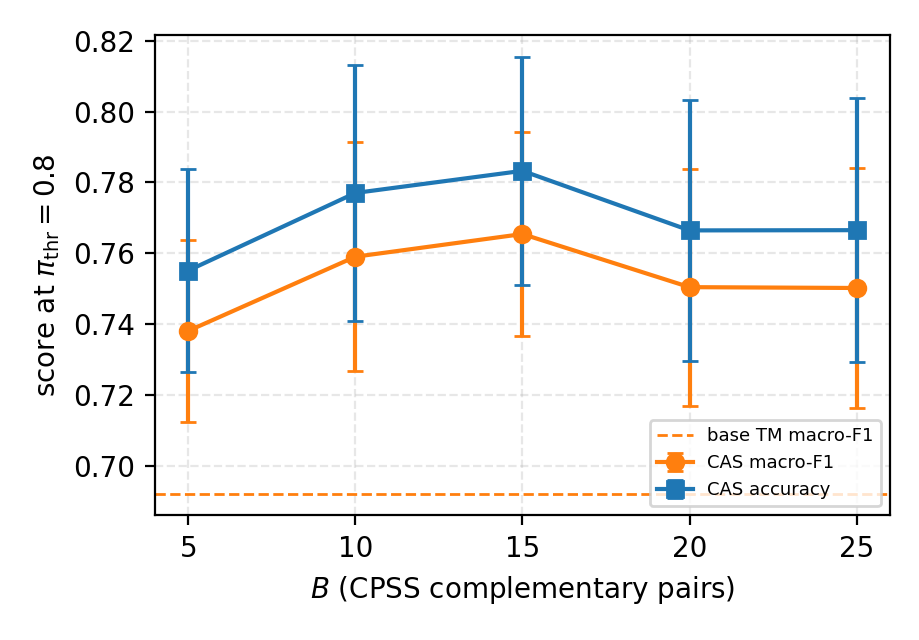
\includegraphics[width=0.49\columnwidth]{old_B.png}
\caption{Sensitivity, three-seed mean$\pm$sd. Left: CAS macro-F1 and
accuracy versus $\pi_{\mathrm{thr}}$ at $B{=}15$; horizontal lines are the
base weighted-TM. Right: versus the number of complementary pairs $B$ at
$\pi_{\mathrm{thr}}{=}0.8$.}
\label{fig:sweep}
\end{figure}

\begin{figure}[!t]
\centering
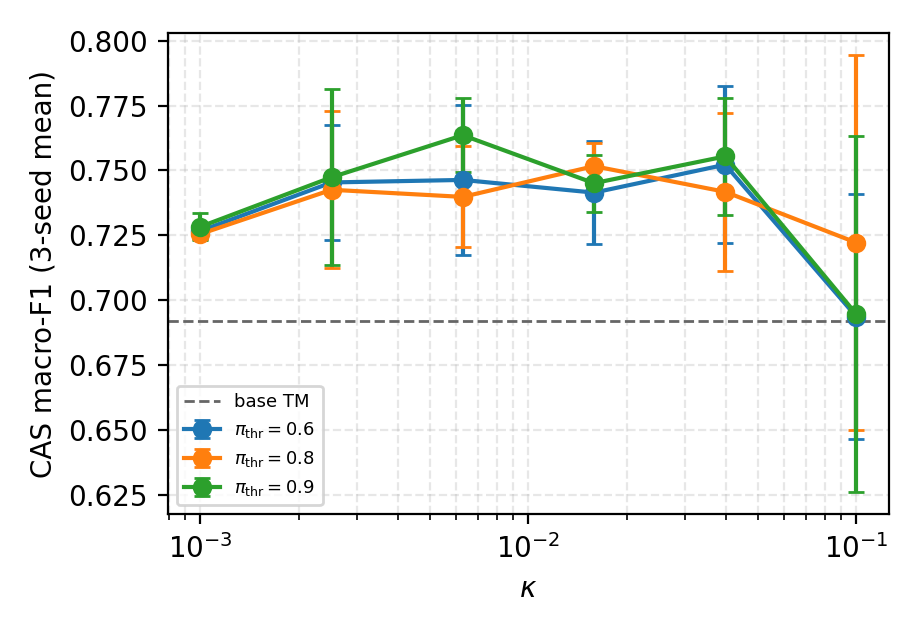
\includegraphics[width=0.70\columnwidth]{old_kappa.png}
\caption{CAS macro-F1 versus the CPSS inverse-regularization strength
$\kappa$ (log axis), one curve per $\pi_{\mathrm{thr}}$, three-seed
mean$\pm$sd. The curve is flat over two decades and only collapses toward
the base detector at $\kappa{=}0.1$.}
\label{fig:kappa}
\end{figure}

\begin{table}[t]
\centering
\caption{$\kappa \times \pi_{\mathrm{thr}}$: three-seed mean CAS macro-F1.
The bottom row is the union-over-grid rule actually used, which dominates
every single $\kappa$ at the verified $\pi_{\mathrm{thr}}{=}0.8$.}
\label{tab:grid}
\small
\begin{tabular}{@{}lccccc@{}}
\toprule
$\kappa \backslash\ \pi_{\mathrm{thr}}$ & 0.5 & 0.6 & 0.7 & 0.8 & 0.9 \\
\midrule
$1.0\!\times\!10^{-3}$ & 0.730 & 0.727 & 0.725 & 0.725 & 0.728 \\
$2.5\!\times\!10^{-3}$ & 0.748 & 0.745 & 0.740 & 0.743 & 0.747 \\
$6.3\!\times\!10^{-3}$ & 0.751 & 0.746 & 0.737 & 0.740 & 0.764 \\
$1.6\!\times\!10^{-2}$ & 0.748 & 0.741 & 0.751 & 0.752 & 0.745 \\
$4.0\!\times\!10^{-2}$ & 0.744 & 0.752 & 0.747 & 0.742 & 0.755 \\
$1.0\!\times\!10^{-1}$ & 0.674 & 0.694 & 0.718 & 0.722 & 0.695 \\
\midrule
union grid (method) & 0.708 & 0.688 & 0.743 & $\mathbf{0.765}$ & 0.762 \\
\bottomrule
\end{tabular}
\end{table}

\subsection{Binary Reduction: The Attack Signature}
\label{sec:binary}
\begin{figure}[!t]
\centering
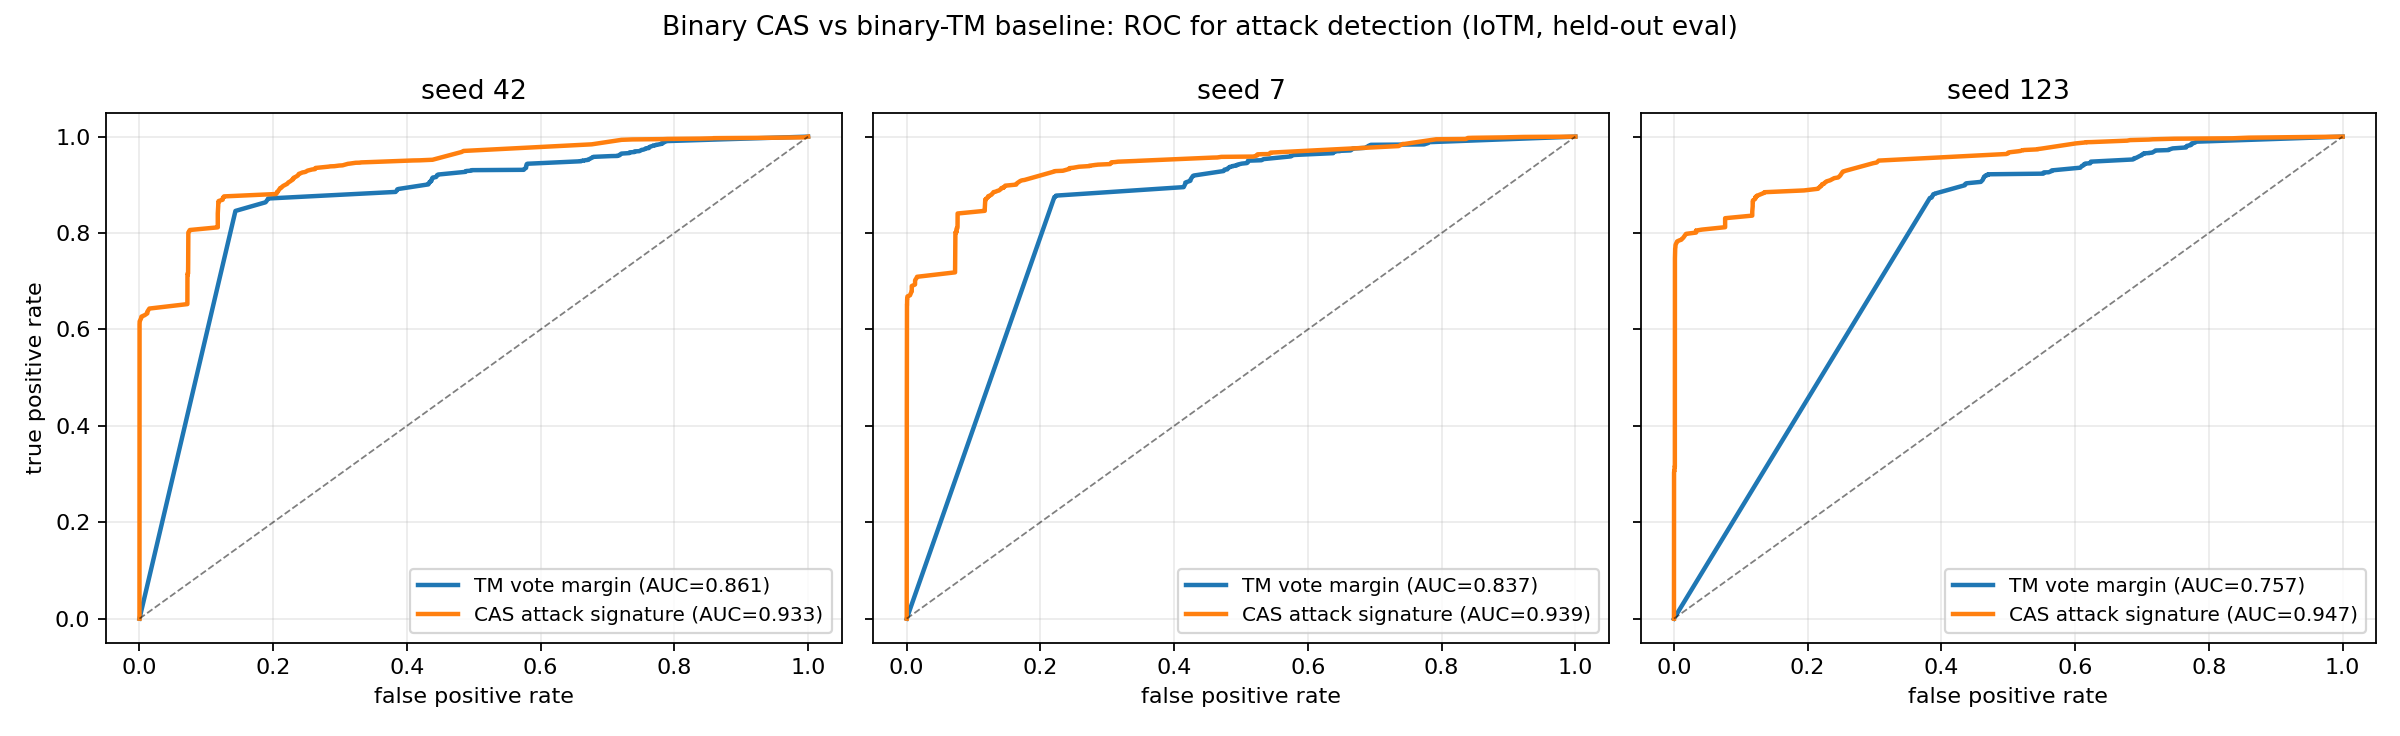
\includegraphics[width=0.44\columnwidth]{binary_cas_roc_iotm.png}
\caption{ROC for attack detection on three seeded binary TMs. The CAS
attack-signature score dominates the TM vote margin on every seed.}
\label{fig:roc}
\end{figure}
Attribution helps only after a flow is flagged malicious, so we next
ask what CAS offers the simpler normal-versus-attack problem: collapsing
the five attack families into one
\textsc{attack} class and training a dedicated two-class TM yields a
binary CAS. Table~\ref{tab:binary} and Fig.~\ref{fig:roc} tell a clear
story. The base TM over-predicts attack: it catches
almost everything (recall 0.988) but cries wolf often (precision 0.847).
The attack signature rebalances the operating point (recall 0.910,
precision 0.947) and, more importantly, ranks flows far better, lifting
AUROC from 0.819 to 0.940. (The binary arm re-binarizes at 5 bins versus
10; each arm is self-consistent.)

\begin{table}[t]
\centering
\caption{Binary attack detection, three seeds (mean).}
\label{tab:binary}
\small
\begin{tabular}{@{}lccc@{}}
\toprule
Method & attack F1 & R / P & AUROC \\
\midrule
Binary TM argmax & $0.912 \pm 0.000$ & 0.988 / 0.847 & 0.819 \\
\textbf{CAS signature} & $\mathbf{0.928 \pm 0.007}$ & 0.910 / 0.947 & \textbf{0.940} \\
\bottomrule
\end{tabular}
\end{table}

\subsection{Signature Content and Certificates}
\label{sec:signatures}
We now open the signatures up:
how compact are they, what do they say, and how much can we trust?
At $\pi_{\mathrm{thr}}{=}0.6$, certified signature size $|S|$ ranges from
115 to 311 clauses, $|S^{+}|$ from 29 to 58, and the $E[V]$ bound from
${\le}72$ to ${\le}250$. At the verified $\pi_{\mathrm{thr}}{=}0.8$
operating point (Table~\ref{tab:reduction}), each family shrinks to just
28--53 sign-positive clauses while F1 \emph{improves} --- compaction and
accuracy are not in tension here.

The content of the signatures is equally reassuring: the decoded DDoS
signature (seed 42) reads like the classic flooding profile: 8 of its 29
sign-positive clauses are high-rate thresholds (\texttt{Rate} $\ge$ 31.5k
packets/s), two more combine high rates with short headers, and two test
for ICMP presence --- matching the SYN-flag pattern found by the binary
attack signature (\S\ref{sec:binary}). Exculpatory lists, conversely, are
dominated by long, low-rate conjunctions that look like benign device
chatter --- an analyst handed these lists would recognize the attack
families from the rules alone.

\begin{table}[t]
\centering
\caption{Signature compaction at the verified operating point (seed 42,
$\pi_{\mathrm{thr}}{=}0.8$). All families start from the same
2{,}400-clause pool.}
\label{tab:reduction}
\small
\begin{tabular}{lccc}
\toprule
Family & Original clauses & Certified $|S|$ & Final $|S^{+}|$ \\
\midrule
Benign   & 2{,}400 & 184 & 41 \\
DDoS     & 2{,}400 &  63 & 29 \\
DoS      & 2{,}400 & 247 & 33 \\
MQTT     & 2{,}400 & 145 & 53 \\
Recon    & 2{,}400 &  66 & 28 \\
Spoofing & 2{,}400 & 194 & 50 \\
\bottomrule
\end{tabular}
\end{table}

That the pool tolerates this much compaction is a property of the trained
TM itself. Solving the pruning program of \S\ref{sec:prune} on these
models, Fig.~\ref{fig:pruning} traces the realised macro-F1 as the budget
$k$ grows in steps of five: it is flat until $335$ of the $400$ clauses
per class ($84\%$ of the pool) are gone, so $\varepsilon = 0.01$ gives
$k^{\star} = 335$.

The surrogate certifies but does not solve~\eqref{eq:prune}, and the slack
is real: allocating the budget more cleverly does not help. Replacing the
uniform per-class $k$ by a global knapsack on $\sum_c R(D_c)$, or by the
minimax rule equalising $\max_c R(D_c)$, changes macro-F1 by less than the
cross-seed spread at matched pool size ($0.689$, $0.678$ and $0.683$ at
$390$ clauses). $R$ is a worst case over inputs that never occur, so
tightening its allocation does not track the realised objective.

\begin{figure}[!t]
\centering
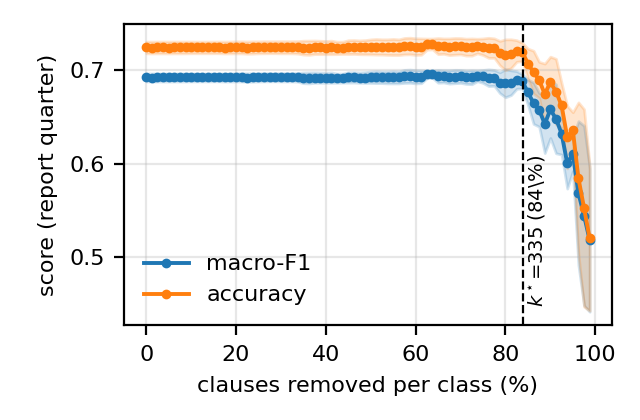
\includegraphics[width=0.70\columnwidth]{clause_pruning.png}
\caption{Clause-weight pruning on the trained weighted TMs, three-seed
mean$\pm$sd on the full test set. Clauses are removed per class in order of
increasing $|$weight$|$, five at a time. Macro-F1 and accuracy are flat
until $84\%$ of the pool has been deleted.}
\label{fig:pruning}
\end{figure}

\subsection{CAS on a Weight-Pruned Pool}
\label{sec:pruned}
The pruning curve suggests an obvious question: if $84\%$ of the pool is
redundant for the base detector, is it also diluting the stability vote?
We therefore keep only the top $65$ clauses per class by $|$weight$|$
--- the knee of Fig.~\ref{fig:pruning} --- and re-run the identical CAS
pipeline on the resulting $390$-clause pool, changing nothing else.

The answer is yes, and by a clear margin (Table~\ref{tab:pruned},
Fig.~\ref{fig:prunedcas}). Pruning costs the base detector nothing
($0.689 \pm 0.008$ vs.\ $0.692 \pm 0.004$), but CAS on the pruned pool
reaches $0.779 \pm 0.025$ --- above the $0.765 \pm 0.029$ obtained from
the full pool --- from signatures of only $26$--$38$ clauses drawn from
$390$ rather than $2{,}400$. More useful than the gain itself is what
happens to the threshold: the full-pool sweep swings from $0.688$ to
$0.765$ depending on $\pi_{\mathrm{thr}}$, whereas the pruned pool is flat
at $0.777$--$0.780$ across the entire range, with roughly half the
cross-seed spread at the top end. The $\pi_{\mathrm{thr}}$ instability
documented in \S\ref{sec:validation} is therefore a property of the
diluted pool, not of CPSS: once the weak clauses are removed, the
stability threshold stops mattering and the method no longer depends on
tuning it.

\begin{table}[t]
\centering
\caption{CAS on the full versus the weight-pruned clause pool, three-seed
macro-F1 at $B{=}15$. Pruning keeps the top 65 clauses per class.}
\label{tab:pruned}
\small
\begin{tabular}{@{}lcc@{}}
\toprule
& full pool ($2{,}400$) & pruned pool ($390$) \\
\midrule
Weighted-TM argmax (base) & $0.692 \pm 0.004$ & $0.689 \pm 0.008$ \\
CAS $\pi_{\mathrm{thr}}{=}0.5$ & $0.708 \pm 0.011$ & $0.777 \pm 0.023$ \\
CAS $\pi_{\mathrm{thr}}{=}0.6$ & $0.688 \pm 0.032$ & $\mathbf{0.779 \pm 0.025}$ \\
CAS $\pi_{\mathrm{thr}}{=}0.7$ & $0.743 \pm 0.015$ & $0.778 \pm 0.023$ \\
CAS $\pi_{\mathrm{thr}}{=}0.8$ & $\mathbf{0.765 \pm 0.029}$ & $0.778 \pm 0.018$ \\
CAS $\pi_{\mathrm{thr}}{=}0.9$ & $0.762 \pm 0.038$ & $0.779 \pm 0.016$ \\
\midrule
mean $|S^{+}|$ at $\pi_{\mathrm{thr}}{=}0.8$ & 43 & 29 \\
\bottomrule
\end{tabular}
\end{table}

\begin{figure}[!t]
\centering
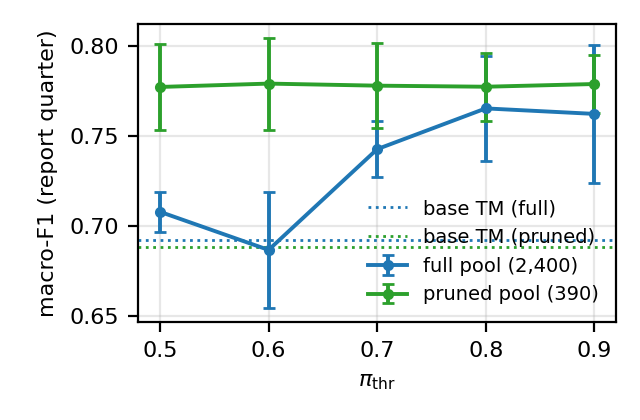
\includegraphics[width=0.70\columnwidth]{pruned_vs_full.png}
\caption{CAS macro-F1 versus $\pi_{\mathrm{thr}}$ on the full and
weight-pruned clause pools, three-seed mean$\pm$sd. Pruning lifts the
curve and flattens it: on the pruned pool the stability threshold no
longer changes the result.}
\label{fig:prunedcas}
\end{figure}

The signatures compact in the same way
(Table~\ref{tab:prunedreduction}): certified sets of $58$--$83$ clauses
and inculpatory cores of $22$--$42$, comparable in absolute size to
Table~\ref{tab:reduction} but drawn from a pool six times smaller, so far
more of what survives pruning is actually used. The $E[V]$ bounds tighten
from ${\le}72$--${\le}250$ to ${\le}27$--${\le}50$, the Shah--Samworth
bound scaling with pool size $p$.

\begin{table}[t]
\centering
\caption{Signature compaction on the weight-pruned pool (seed 42,
$\pi_{\mathrm{thr}}{=}0.8$, $B{=}15$). All families start from the same
$390$-clause pool; compare Table~\ref{tab:reduction}.}
\label{tab:prunedreduction}
\small
\begin{tabular}{lcccc}
\toprule
Family & Original clauses & Certified $|S|$ & Final $|S^{+}|$ & $E[V]$ \\
\midrule
Benign   & 390 & 63 & 30 & ${\le}32$ \\
DDoS     & 390 & 66 & 36 & ${\le}27$ \\
DoS      & 390 & 83 & 42 & ${\le}38$ \\
MQTT     & 390 & 64 & 26 & ${\le}30$ \\
Recon    & 390 & 58 & 22 & ${\le}41$ \\
Spoofing & 390 & 76 & 28 & ${\le}50$ \\
\bottomrule
\end{tabular}
\end{table}

\subsection{Task B: Open-Set Behavior (Leave-One-Family-Out)}
\label{sec:taskb}
A deployed detector will meet attacks it has never seen, so we
stress-test CAS leave-one-family-out: hold out one
family, retrain, and calibrate split-conformal novelty thresholds
($\epsilon{=}0.05$, two folds). The result is honestly negative: the
false-flag guarantee holds in both folds (FPR 0.035 Spoofing, 0.027 MQTT,
under target), but
detection power against novel families is weak: Spoofing AUROC is 0.275,
below chance, and MQTT reaches only 0.622 (Fig.~\ref{fig:taskb}). The
reason is instructive: ARP-spoofing traffic
closely resembles legitimate ARP-based device discovery in this feature
space --- a measured blind spot.

\begin{figure}[!t]
\centering
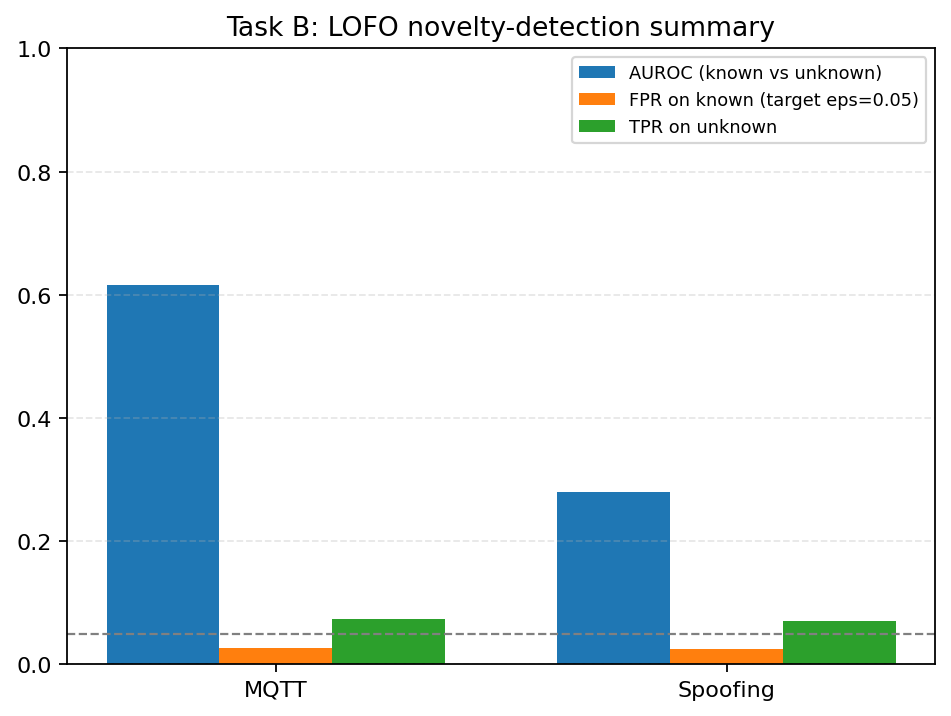
\includegraphics[width=0.30\columnwidth]{task_b_lofo_summary.png}
\caption{Leave-one-family-out: conformal false-flag rates stay under
target, but novelty AUROC against the held-out family is weak.}
\label{fig:taskb}
\end{figure}

\subsection{Signature Identifiability: Disjunct Certificates}
\label{sec:disjunct}
The next question is combinatorial: if several attack families are active
at once, can the signatures still be told apart? Arrange the six
inculpatory signatures as columns of a binary clause-by-family table; the
table is $t$-disjunct when no column is covered by the union of any $t$
others, so every family keeps a unique mark under up to $t$
simultaneous others. Computing the largest such $t$ exactly gives
$\hat{t}=5$ on every seed and both thresholds --- the maximum possible
with six families --- so any mixture of up to five families decodes
exactly when there is no noise.

Noise, however, separates the code from the decoder
(500 trials per setting, three seeds): the
strict COMP decoder recovers every mixture noiselessly, but collapses to
0.2\%--1.8\% under 5\% bit-flip noise, while a thresholded variant that
accepts partial matches restores 99.8\%--100\% decoding at threshold 0.8
(85\%--90\% at 0.9) and still reaches 68\%--76\% at 15\% noise. Overlap
reduction itself removes only 11--22 clauses from the pool. The code is
strong; the decoder needs care under noise.

\subsection{Cross-Seed Stability: A Negative Result}
\label{sec:stability}
We close with a limitation: across the three seeded TMs, the pairwise
Kuncheva index on
clause-index overlap sits near zero for every family ($-0.015$ to
$0.111$; Fig.~\ref{fig:kuncheva}): identically numbered clauses in
different seeds are
unrelated learned rules, so CAS stabilizes
selection \emph{within}
a trained TM; signature identity does not survive retraining.

\begin{figure}[!t]
\centering
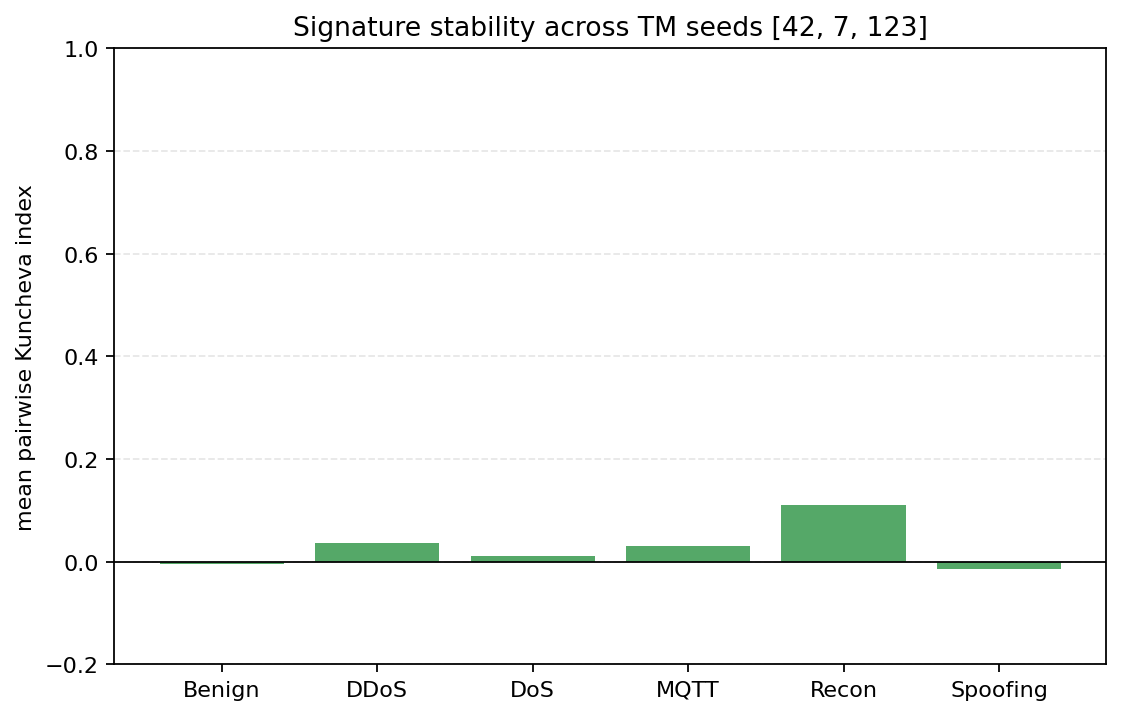
\includegraphics[width=0.30\columnwidth]{stability_kuncheva.png}
\caption{Pairwise Kuncheva index on clause-index overlap between seeded
TMs: near zero for every family.}
\label{fig:kuncheva}
\end{figure}

\section{Discussion}
\label{sec:discussion}
CAS improves on its base TM when the base still has headroom; a
near-ceiling base would turn the same construction into lossy
compression, so we position CAS as an attribution layer over a weak base
detector. CICIoMT2024
models can suffer large cross-dataset F1 drops~\cite{domenech2025}; our
claims remain single-dataset and transfer is open. Limitations: (i) no
post-hoc XAI baseline (SHAP, Anchors) yet; (ii) loose $E[V]$ bounds;
(iii) instability at $\pi_{\mathrm{thr}}{=}0.6$ on the full pool, which
weight-pruning removes (\S\ref{sec:pruned}); (iv) weak
cross-seed signature identity (\S\ref{sec:stability}); (v) synthetic
OR-mixtures, not real traffic, in disjunct decoding.

\section{Conclusion}
CAS turns the clause pool of a trained TM into compact signed evidence
lists per family, with a bound on spurious inclusions and exact mixture
identifiability. On CICIoMT2024 it beats its base detector (macro-F1
0.765 vs.\ 0.692; binary AUROC 0.940); open-set
and cross-seed limits bound the claim.

\begin{thebibliography}{15}
\bibitem{granmo2018} O.-C. Granmo, ``The Tsetlin Machine --- a
game-theoretic bandit-driven approach to optimal pattern recognition with
propositional logic,'' \emph{arXiv:1804.01508}, 2018.
\bibitem{phoulady2020} O.-C. Granmo and S. Phoulady, ``The Weighted Tsetlin
Machine,'' \emph{arXiv:2002.01245}, 2020.
\bibitem{jaiswal2026iomt} R. Jaiswal, P.-A. Andersen, L. R. Cenkeramaddi,
L. Jiao, and O.-C. Granmo, ``A Tsetlin Machine-driven Intrusion Detection
System for Next-Generation IoMT Security,'' \emph{IEEE SVCC} /
\emph{arXiv:2604.03205}, 2026.
\bibitem{shah2013} R. Shah and R. Samworth, ``Variable selection with error
control: another look at stability selection,'' \emph{JRSS-B}, vol. 75,
no. 1, pp. 55--80, 2013.
\bibitem{tmu} O.-C. Granmo et al., ``TMU: Tsetlin Machine Unified,''
github.com/cair/tmu.
\bibitem{abeyrathna2020} K. D. Abeyrathna et al., ``Intrusion Detection
with Interpretable Rules Generated using the Tsetlin Machine,'' \emph{IEEE
SSCI}, 2020.
\bibitem{jaiswal2026medsec} R. Jaiswal et al., ``On-Device Interpretable
Tsetlin Machine-Based Intrusion Detection for Secure IoMT,''
\emph{arXiv:2605.16707}, 2026.
\bibitem{meinshausen2010} N. Meinshausen and P. B\"uhlmann, ``Stability
selection,'' \emph{JRSS-B}, vol. 72, no. 4, pp. 417--473, 2010.
\bibitem{sommer2010} R. Sommer and V. Paxson, ``Outside the Closed World: On
Using Machine Learning for Network Intrusion Detection,'' \emph{IEEE S\&P},
2010.
\bibitem{engelen2021} G. Engelen, V. Rimmer, and W. Joosen,
``Troubleshooting an Intrusion Detection Dataset: the CICIDS2017 Case
Study,'' \emph{IEEE SPW}, 2021.
\bibitem{arp2022} D. Arp et al., ``Dos and Don'ts of Machine Learning in
Computer Security,'' \emph{USENIX Security}, 2022.
\bibitem{dadkhah2024} S. Dadkhah et al., ``CICIoMT2024: A benchmark dataset
for multi-protocol security assessment in IoMT,'' \emph{Internet of Things},
vol. 28, art. 101351, 2024.
\bibitem{domenech2025} J. Dom\'enech Fons, ``Evaluating and enhancing
intrusion detection systems in IoMT: The importance of domain-specific
datasets,'' \emph{Internet of Things}, 2025.
\bibitem{xaiids2025} ``Explainable AI for Interpreting ML-based IDS using
LIME and SHAP,'' \emph{Applied Sciences}, vol. 15, no. 13, 2025.
\bibitem{du1993} D.-Z. Du and F. K. Hwang, \emph{Combinatorial Group Testing
and Its Applications}, World Scientific, 1993.
\end{thebibliography}

\end{document}
